% THIS DOCUMENT IS FOLLOWS THE VOLERE TEMPLATE BY Suzanne Robertson and James Robertson
% ONLY THE SECTION HEADINGS ARE PROVIDED
%
% Initial draft from https://github.com/Dieblich/volere
%
% Risks are removed because they are covered by the Hazard Analysis
\documentclass[12pt, titlepage]{article}
\usepackage[parfill]{parskip}

%\usepackage[pdftex]{graphicx}
%\graphicspath{{../pdf/}{D:\ImagesforProjectLatex}}
 %\DeclareGraphicsExtensions{.pdf,.jpeg,.png}
\usepackage{graphicx}
\usepackage{makecell}
\usepackage{amsmath}
\usepackage{booktabs}
\usepackage{tabularx}
\usepackage{hyperref}
\usepackage{float} 
\usepackage{longtable}
\hypersetup{
    bookmarks=true,         % show bookmarks bar?
      colorlinks=true,      % false: boxed links; true: colored links
    linkcolor=red,          % color of internal links (change box color with linkbordercolor)
    citecolor=green,        % color of links to bibliography
    filecolor=magenta,      % color of file links
    urlcolor=cyan           % color of external links
}

\newcommand{\lips}{\textit{Insert your content here.}}

%% Comments

\usepackage{color}

\newif\ifcomments\commentstrue %displays comments
%\newif\ifcomments\commentsfalse %so that comments do not display

\ifcomments
\newcommand{\authornote}[3]{\textcolor{#1}{[#3 ---#2]}}
\newcommand{\todo}[1]{\textcolor{red}{[TODO: #1]}}
\else
\newcommand{\authornote}[3]{}
\newcommand{\todo}[1]{}
\fi

\newcommand{\wss}[1]{\authornote{blue}{SS}{#1}} 
\newcommand{\plt}[1]{\authornote{magenta}{TPLT}{#1}} %For explanation of the template
\newcommand{\an}[1]{\authornote{cyan}{Author}{#1}}

%% Common Parts

\newcommand{\progname}{ProgName} % PUT YOUR PROGRAM NAME HERE
\newcommand{\authname}{Team \#, Team Name
\\ Student 1 name
\\ Student 2 name
\\ Student 3 name
\\ Student 4 name} % AUTHOR NAMES                  

\usepackage{hyperref}
    \hypersetup{colorlinks=true, linkcolor=blue, citecolor=blue, filecolor=blue,
                urlcolor=blue, unicode=false}
    \urlstyle{same}
                                


\begin{document}

\title{Software Requirements Specification for \progname: McMaster Graduate Softball League Management Platform} 
\author{\authname}
\date{\today}
	
\maketitle

~\newpage

\pagenumbering{roman}

\tableofcontents

\listoftables

~\newpage

\section*{Revision History}

\begin{tabularx}{\textwidth}{p{3cm}p{2cm}X}
\toprule {\textbf{Date}} & {\textbf{Version}} & {\textbf{Notes}}\\
\midrule
April 3, 2024 & 1.1 & Major revision based on feedback and requirements changes (refer to Revision 1 Traceability table for details )\\
Oct 11, 2023 & 1.0 & Initial Creation \\
\bottomrule
\end{tabularx}

~\\

~\newpage

\subsection{Revision 1 Traceability}
The following table tracks all significant changes made to the SRS based on feedback, requirements changes, and improvements:

\begin{longtable}{|p{0.15\textwidth}|p{0.35\textwidth}|p{0.2\textwidth}|p{0.2\textwidth}|}
\caption{Traceability of Revision 1 Changes} \label{tab:revision_traceability} \\
\hline
\textbf{Change ID} & \textbf{Description of Change} & \textbf{Affected Section(s)} & \textbf{GitHub Issue} \\
\hline
\endfirsthead

\multicolumn{4}{c}{\tablename\ \thetable{} -- Continued from previous page} \\
\hline
\textbf{Change ID} & \textbf{Description of Change} & \textbf{Affected Section(s)} & \textbf{GitHub Issue} \\
\hline
\endhead

\hline \multicolumn{4}{r}{Continued on next page} \\
\endfoot

\hline
\endlastfoot

REV1.1 & Modified team joining process: Only captains can invite players & Functional Requirements \#6 & Issue \#468 \\
\hline
REV1.2 & Enhanced schedule view requirements: Added specific views & Functional Requirements \#3 & Issue \#469 \\
\hline
REV1.3 & Added player profile page requirement & Functional Requirements & Issue \#470 \\
\hline
REV1.4 & Update requirements to align with HA document & Non-Functional Requirements & Issue \#473 \\
\hline
REV1.5 & Added formal specifications with state machine model & Formal Specifications & Issue \#474 \\
\hline
REV1.6 & Enhanced data dictionary with detailed attributes & Business Data Model & Issue \#476 \\
\hline
REV1.7 & Expanded introduction with clearer context & Introduction & Issue \#478 \\
\hline
REV1.8 & Implemented consistent requirement numbering (UC1, FR1, NFR-LF1) & All Requirements & Issue \#477 \\
\hline
REV1.9 & Replaced magic numbers with symbolic constants & All & Issue \#471 \\
\hline
REV1.10 & Added introductory text to all sections & All & Issue \#485 \\
\hline
REV1.11 & Added comprehensive traceability matrices & Traceability & Issue \#486 \\
\hline
REV1.12 & Enhanced diagram descriptions and references & All & Issue \#487 \\
\hline
REV1.13 & Add hyperlinks to table and figure references & All & Issue \#488 \\
\hline
REV1.14 & Enhanced persona descriptions & Stakeholders & Issue \#489 \\
\hline
REV1.15 & Added quantifiable fit criteria to NFRs & Non-Functional Requirements & Issue \#472 \\
\hline
REV1.16 & Identify requirements that are likely/unlikely to change & Likely Changes & Issue \#505 \\
\hline
REV1.17 & Identify template and changes made & Template Information & Issue \#506 \\
\hline
\end{longtable}

\section{Template Information}
This section documents the template used and modifications made to create this SRS document.

\subsection{Template Source}
This document follows the Volere Requirements Specification Template by Suzanne Robertson and James Robertson. The initial draft was adapted from \url{https://github.com/Dieblich/volere}, with significant modifications to suit the needs of the McMaster GSA softball league platform project.

\subsection{Major Template Modifications}
The following significant modifications were made to the original Volere template:

\begin{enumerate}
    \item \textbf{Removed Sections}
    \begin{itemize}
        \item Risks section removed as it is covered in the separate Hazard Analysis document
        \item Cost estimates section simplified due to academic nature of project
        \item Solution constraints section modified to focus on technical constraints
    \end{itemize}

    \item \textbf{Added Sections}
    \begin{itemize}
        \item Comprehensive symbolic parameters table for configuration values
        \item Detailed traceability matrices linking requirements, use cases, and hazards
        \item Formal specifications section with state machine model
    \end{itemize}
\end{enumerate}

\section{Purpose of the Project}
This section outlines the core business objectives and goals of the McMaster GSA softball league platform, detailing how the system will serve its users and enhance league operations.
\subsection{User Business}
The primary business of the McMaster GSA softball league is to facilitate recreational softball activities for students, staff, and alumni. The league aims to provide an organized platform for scheduling games, managing teams, and tracking player performance, enhancing the overall experience for participants. By streamlining league operations, the platform will foster a more inclusive and efficient environment, enabling better communication among players, captains, and commissioners.\
\begin{itemize}
  \item Team Management: captains will have the ability to create and manage their teams, inviting players to join, assigning roles, and ensuring that all team members are informed about practices and games.
  \item Game Scheduling: users will utilize the scheduling tools to view upcoming games, propose new times, and request rescheduling, ensuring that all participants are aware of their commitments and can manage their time effectively.
  \item Communication and Announcements: Commissioners will post league-wide announcements and updates, allowing all users to stay informed about important news, such as changes in scheduling, league policies, or events.
  \item Performance Tracking: players can track their individual and team performance through leaderboards and standings, fostering a sense of competition and motivation to improve.
  \item Payment Management: the application will provide visibility into players' payment statuses, enabling captains and commissioners to easily monitor team compliance with league participation requirements.
  \item Community Building: through features such as announcements and event notifications, users can engage with one another beyond the field, strengthening community ties and enhancing the overall experience of league participation.
\end{itemize}
\subsection{Goals of the Project}
The primary goal of the McMaster GSA softball league platform project is to develop an intuitive, user-friendly web application that enhances the management and operation of the league. Specific goals include:
\begin{itemize}
  \item Streamlined Scheduling and Communication: Simplify the scheduling process for games and practices, allowing captains to manage their teams effectively while facilitating clear communication between all stakeholders.
  \item Role-Based Access Control (RBAC): Use a secure login system that allows different levels of access for different users, ensuring that users can perform actions relevant to their roles without compromising sensitive information.
  \item Improved User Interface: Design a modern, responsive user interface that enhances usability and engagement, making it easier for participants to navigate the platform and access essential features.
  \item Enhanced Data Management: Develop robust features for managing player registrations, tracking payment statuses, and maintaining accurate standings and leaderboards, thereby reducing administrative overhead and increasing transparency.
  \item Facilitate Community Engagement: Foster a sense of community among participants through features such as announcements, event notifications, and an organized platform for sharing updates, enhancing the overall experience of league participation.
\end{itemize}

\pagebreak

\section{Stakeholders}
This section identifies and describes the key stakeholders who will interact with or be affected by the platform, including their roles, needs, and expectations.
\subsection{Client}
The client for this project is the McMaster GSA, which oversees the softball league. Their primary goal is to provide a robust platform that improves the management of the league, facilitates better communication among users, and enhances the overall user experience. The GSA will benefit from increased participation and smoother operations, ultimately fostering a stronger community at McMaster.
\subsection{Customer}
The customers are the users of the platform, including players, captains, and commissioners. They seek an intuitive and efficient system that allows for easy management of games, team coordination, and communication. By addressing their needs, the platform aims to increase user satisfaction and engagement within the league.
\subsection{Other Stakeholders}
Other stakeholders include the university administration, potential sponsors, and the broader McMaster University community. These groups may have a vested interest in the successful operation of the league, as it contributes to student life and community engagement. Sponsors may seek visibility and promotional opportunities through the league's activities.
\subsection{Hands-On Users of the Project}
Hands-on users include the players, captains, and commissioners who will interact with the platform daily. Players will use the system to join teams, view schedules, and track their performance. Captains will manage their teams, schedule games, and communicate with players. Commissioners will oversee league operations, post announcements, and manage administrative tasks.
\subsection{Personas}
\begin{itemize}
    \item \textbf{Player Persona - Margaret Simon}
    \begin{itemize}
        \item \textbf{Background:} 2nd-year Masters student in Chemical Engineering
        \item \textbf{Technical Proficiency:} Moderate, comfortable with basic web applications
        \item \textbf{Goals:}
        \begin{itemize}
            \item Find and join a team that matches her skill level
            \item Easily check game schedules around her lab work
            \item Track her team's progress throughout the season
        \end{itemize}
        \item \textbf{Pain Points:}
        \begin{itemize}
            \item Limited time due to academic commitments
        \end{itemize}
    \end{itemize}

    \item \textbf{Captain Persona - Nancy Wheeler}
    \begin{itemize}
        \item \textbf{Background:} PhD candidate in Physics, 3rd year as team captain
        \item \textbf{Technical Proficiency:} High, experienced with various software tools
        \item \textbf{Goals:}
        \begin{itemize}
            \item Efficiently manage team roster and communications
            \item Handle game scheduling and rescheduling requests
            \item Track team performance and player attendance
        \end{itemize}
        \item \textbf{Pain Points:}
        \begin{itemize}
            \item Coordinating multiple players' schedules
            \item Needs streamlined communication tools
            \item Requires quick access to league rules and policies
        \end{itemize}
    \end{itemize}

    \item \textbf{Commissioner Persona - Dr. Philip Leroy}
    \begin{itemize}
        \item \textbf{Background:} Postdoctoral researcher, 5+ years league experience
        \item \textbf{Technical Proficiency:} Moderate to high, focuses on efficiency
        \item \textbf{Goals:}
        \begin{itemize}
            \item Oversee league operations and maintain fairness
            \item Manage schedule conflicts and weather-related changes
            \item Ensure clear communication of league policies
        \end{itemize}
        \item \textbf{Pain Points:}
        \begin{itemize}
            \item Handling multiple rescheduling requests
            \item Needs efficient tools for league-wide announcements
            \item Requires clear oversight of all team activities
        \end{itemize}
    \end{itemize}
\end{itemize}
\subsection{Priorities Assigned to Users}
Players prioritize ease of joining teams, checking their game schedule, and tracking performance.
Captains focus on scheduling flexibility, team management features, and communication tools.
Commissioners prioritize administrative functionality, announcement features, and overall system reliability.
\subsection{User Participation}
User participation will be critical throughout the project. Stakeholders will provide feedback during the development process to ensure the platform meets their needs. User testing sessions will be conducted to gather insights and refine the interface and features.
\subsection{Maintenance Users and Service Technicians}
Maintenance users include any staff responsible for ongoing system updates, bug fixes, and technical support (our team). This group ensures that the platform remains functional, secure, and up-to-date. Service technicians may be involved in troubleshooting issues and providing assistance to users, particularly during peak usage periods, such as the beginning of the season.

\section{Mandated Constraints}

\subsection{Solution Constraints}
Constraints that limit the design of the solution:
\begin{itemize}
    \item \textbf{Scalability}: The initial version of the platform must support \hyperref[MIN_TEAMS]{\texttt{MIN\_TEAMS}} to \hyperref[MAX_TEAMS]{\texttt{MAX\_TEAMS}} teams, with future scalability to accommodate more teams.
    \item \textbf{Device Accessibility}: The system must be optimized for desktops, tablets, and mobile phones.
\end{itemize}

\subsection{Implementation Environment of the Current System}
The current implementation environment includes:
\begin{itemize}
    \item \textbf{Operating Systems}: Compatibility with Windows, macOS, Android, and iOS.
    \item \textbf{Supported Browsers}: The platform must be fully functional on Chrome, Firefox, Safari, and Edge.
    \item \textbf{Hosting Environment}: The platform will continue to use the existing hosting environment, which has already been established for the current website. No changes to the hosting infrastructure are anticipated unless new features require additional support.
\end{itemize}

\subsection{Partner or Collaborative Applications}
There are no partner or collaborative applications required for this project.

\subsection{Off-the-Shelf Software}
No off-the-shelf software will be utilized for payment handling or calendar integration.

\subsection{Anticipated Workplace Environment}
The platform is anticipated to be used in various environments:
\begin{itemize}
    \item \textbf{Users}: The platform will be accessed by league commissioners, team captains, players, and administrators.
    \item \textbf{Device Types}: Users are expected to use the platform on personal laptops, desktops, and mobile devices.
\end{itemize}

\subsection{Schedule Constraints}
The project is constrained by a strict timeline, with key milestones that must be met:
\begin{itemize}
    \item \textbf{Development Timeline}: The platform must be completed within the designated course timeline (approximately 8 months).
    \item \textbf{Fixed Milestones}: Deliverables must be submitted according to predefined deadlines.
\end{itemize}

\subsection{Budget Constraints}
There are no budget constraints applicable to this project. The existing infrastructure and hosting environment will be reused, and no additional licensing fees are required.

\subsection{Enterprise Constraints}
\begin{itemize}
    \item \textbf{Hosting Environment}: The platform must utilize the existing hosting environment already set up for the current system, which may come with certain limitations or capabilities that need to be respected.
    \item \textbf{No External Sponsorship}: There is no specific enterprise funding or sponsoring this project, meaning there are no additional budgetary or compliance constraints from an external organization.
\end{itemize}

\section{Naming Conventions and Terminology}

\subsection{Glossary of All Terms, Including Acronyms, Used by Stakeholders involved in the Project}
The following terms are used consistently throughout this document:
\begin{itemize}
    \item \textbf{Commissioner}: Manages the entire league and oversees operations.
    \item \textbf{Captain}: Responsible for team management, including schedules and rosters.
    \item \textbf{Player}: A participant in a team who needs access to schedules and standings.
    \item \textbf{Schedule Slot}: The specific time allocated for a game.
    \item \textbf{Waiver}: A document that participants must sign before joining the league.
\end{itemize}

\section{Relevant Facts and Assumptions}

\subsection{Relevant Facts}
\begin{itemize}
    \item \textbf{Role Definition}: Specific roles such as commissioner, captain, and player exist within the system, each with unique permissions and responsibilities.
    \item \textbf{Season Timeline}: The platform will primarily be used during the softball season from April to September.
\end{itemize}

\subsection{Business Rules}
\begin{itemize}
    \item \textbf{Team Registration}: Teams must be registered by captains before the league starts.
    \item \textbf{Scheduling Requests}: Rescheduling requests must be made at least \hyperref[RESCHEDULE_NOTICE_HOURS]{\texttt{RESCHEDULE\_NOTICE\_HOURS}} hours in advance.
\end{itemize}

\subsection{Assumptions}
\begin{itemize}
    \item \textbf{Internet Access}: All users are assumed to have access to a stable internet connection.
    \item \textbf{Mobile Usage}: It is assumed that many users will access the platform using mobile devices, so a mobile-friendly interface is required.
    \item \textbf{Payment Compliance}: Players are expected to make payments via e-transfer, which will be managed externally. The platform will include an interface for the designated staff member to track which players have completed their payments, without integrating any direct payment gateway. Manually updated payment status is assumed to be correct.
\end{itemize}

\section{The Scope of the Work}
\subsection{The Current Situation}
The current implementation of the GSA softball league platform is run on outdated software.
This issue makes the management of the league platform difficult without a certain degree of
programming knowledge. The purpose of the GSA softball platform is to manage the softball
league functionalities (communication, scheduling, player logins, etc.) so it meets the needs
and demands of the league.
\subsection{The Context of the Work}
The GSA Softball League Platform interacts with various external entities including players, captains, commissioners, and integrated systems. The system context diagram below illustrates these interaction boundaries, data flows, and system interfaces, highlighting the scope of the platform's functionality and its relationships with users and external systems. See \hyperref[fig:context_diagram]{Figure~\ref{fig:context_diagram}} for the system context diagram.

\begin{figure}[H]
    \centering
    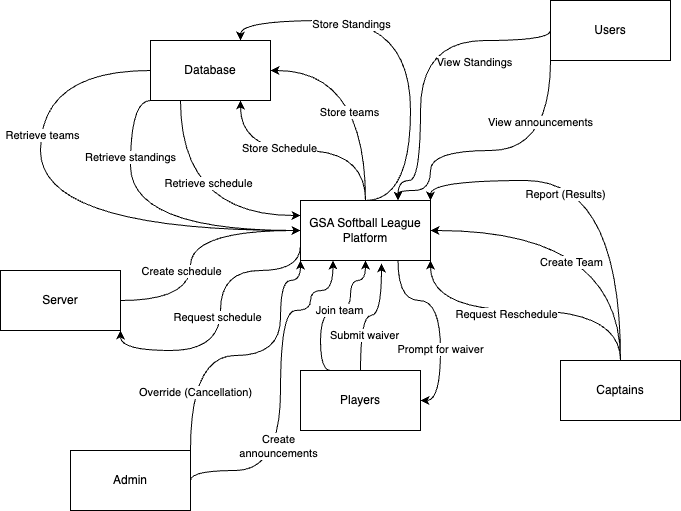
\includegraphics[width=\linewidth]{Context_diagram.png}
    \caption{System Context Diagram}
    \label{fig:context_diagram}
\end{figure}
\pagebreak
\subsection{Work Partitioning}
\begin{center}
    \begin{tabular}{ |c|c|c| }
        \hline
        \textbf{Event Name}  & \textbf{Input/Output} & \textbf{Summary} \\
        \hline
        Login & \makecell{User ID (IN) \\ Password (IN)}
		& \makecell{Enter user ID and password.
		\\User is created and user data
		\\is stored in the database.} \\
        \hline
		Join team & \makecell{User Login (IN) \\ Prompt for waiver (OUT) \\ Submit waiver (IN)}
		& \makecell{User logs in as a player, then
		\\completing the waiver allows
		\\the user to join a team} \\
		\hline
        Create team & \makecell{User Login (IN) \\ Team Info (IN)}
		& \makecell{User logins into the system as
		\\a captain, then the user inputs
		\\the team info to create a team.
		\\The team is created and stored
		\\in the database.} \\
		\hline
        Create Schedule & Season Schedule (OUT)
		& \makecell{System uses all teams info to
		\\create season-long schedule
		\\with all open slots available.} \\
		\hline
        Override & Admin credentials (IN)
		& \makecell{User inputs admin credentials
		\\and gets access to complete
		\\override.} \\
		\hline
        Create announcement & \makecell{Admin credentials (IN)
		\\Announcement details (IN) \\Publish announcement (OUT)}
		& \makecell{User inputs admin credentials
		\\to gain access then enters
		\\in the announcements details.
		\\Then the announcement is
		\\published on the web page.} \\
		\hline
        Request reschedule & User Login (IN) 
		& \makecell{User logs into the system as
		\\a captain, then creates a
		\\request to reschedule a game
		\\in an open slot.}\\
		\hline
        Report (Results) & \makecell{User Login (IN)
		\\ Game results (IN) \\ Update standings (OUT)}
		& \makecell{User logs in as a captain then
		\\inputs the results of the game.
		\\Update standings in the database
		\\with reported results.} \\
        \hline
    \end{tabular}
\end{center}

\subsection{Specifying a Business Use Case}
The primary business use case for this platform is to efficiently manage all aspects of league operations from player registrations to game scheduling in a user-friendly and streamlined manner. The platform will provide commissioners, team captains, and players with a centralized system to interact with the league. The system allows commissioners to oversee the entire league, manage team and player information, and handle payments. Team captains will be able to manage their rosters, submit rescheduling requests, and report game scores, while players can join teams, view schedules, and observe league rankings and scores.
For example, team captains can log in to the platform and create their teams. Players can join a team by requesting approval from the captain, while commissioners can monitor the overall progress and approve team formations. Throughout the season, captains can report game scores directly into the system, which automatically updates the standings. If a team needs to reschedule a game, the captain can request a change through the system, selecting from available timeslots. The system will queue the request for commissioner approval and update the schedule once the rescheduling is confirmed.

\section{Business Data Model and Data Dictionary}
\subsection{Business Data Model}
\begin{itemize}
    \item \textbf{User}
    \begin{itemize}
        \item UserID: Unique identifier for each user.
        \item Name: Full name of the user.
        \item Email: Email address used for communication and login.
        \item Role: The role of the user in the system (commissioner, captain, player).
        \item TeamID: The ID of the team the user is affiliated with (for captains and players).
    \end{itemize}
    
    \item \textbf{Team}
    \begin{itemize}
        \item TeamID: Unique identifier for each team.
        \item TeamName: Name of the team.
        \item Division: The division the team is assigned to.
        \item CaptainID: The UserID of the team captain.
        \item Roster: List of players (UserIDs) on the team.
    \end{itemize}
    
    \item \textbf{Game}
    \begin{itemize}
        \item GameID: Unique identifier for each game.
        \item TeamAID: The ID of the first participating team.
        \item TeamBID: The ID of the second participating team.
        \item Date: The date the game is scheduled.
        \item Time: The time the game is scheduled.
        \item Result: The outcome of the game (win/loss/tie) reported by captains.
        \item ScoreTeamA: The score of Team A in the game.
        \item ScoreTeamB: The score of Team B in the game.
    \end{itemize}
    
    \item \textbf{Schedule}
    \begin{itemize}
        \item ScheduleID: Unique identifier for the schedule.
        \item GameID: The ID of the game scheduled.
        \item SlotNumber: The slot number for the game (time and location).
        \item AvailableSlots: List of available time slots for potential rescheduling.
    \end{itemize}
    
    \item \textbf{Standing}
    \begin{itemize}
        \item TeamID: The ID of the team.
        \item Wins: Number of games won by the team.
        \item Losses: Number of games lost by the team.
        \item Ties: Number of tied games.
        \item Rank: Current rank of the team in the league.
        \item TotalScore: Cumulative score across all games, used to break ties in standings.
    \end{itemize}
\end{itemize}

\subsection{Data Dictionary}
\begin{itemize}
    \item \textbf{Users:} There are three types of users: commissioners, team captains, and players. Commissioners oversee league operations, team captains manage their respective teams, and players join and participate in games. Each user has attributes such as name, email, role, and team affiliation.
    
    \item \textbf{Teams:} Teams consist of players and a captain. Teams are scheduled to play games, and the results of those games contribute to league standings. Teams have attributes like team name, captain, and roster.
    
    \item \textbf{Games:} Games represent the scheduled matches between two teams. Each game has attributes like date, time, and the teams involved, as well as the final score for both teams, which is reported by captains after the game.
    
    \item \textbf{Schedules:} The schedule defines the timing and location of games. It also includes available time slots for rescheduling. The system tracks preferences for game days and times, and generates the schedule accordingly.
    
    \item \textbf{Standings:} Standings reflect the rankings of teams based on the results of their games. Game scores feed into the standings, updating the number of wins, losses, and ties for each team, which determine the overall ranking.
\end{itemize}

\section{Formal Specifications}
\subsection{State Machine Model}
The system can be modeled as a state machine with the following states and transitions:

\begin{itemize}
    \item \textbf{States:}
    \begin{itemize}
        \item $S_0$: Initial state (not logged in)
        \item $S_1$: Logged in as Player
        \item $S_2$: Logged in as Captain
        \item $S_3$: Logged in as Commissioner
        \item $S_4$: Team Creation
        \item $S_5$: Game Scheduling
        \item $S_6$: Score Reporting
    \end{itemize}

    \item \textbf{Transitions:}
    \begin{itemize}
        \item $T_{0,1}$: Login as Player
        \item $T_{0,2}$: Login as Captain
        \item $T_{0,3}$: Login as Commissioner
        \item $T_{2,4}$: Create Team
        \item $T_{2,5}$: Schedule Game
        \item $T_{2,6}$: Report Score
        \item $T_{1,0}$: Logout
        \item $T_{2,0}$: Logout
        \item $T_{3,0}$: Logout
    \end{itemize}

    \item \textbf{State Invariants:}
    \begin{itemize}
        \item $\forall s \in S: s \neq S_0 \implies \text{user is authenticated}$
        \item $\forall s \in \{S_4, S_5, S_6\}: s \implies \text{user has appropriate permissions}$
    \end{itemize}
\end{itemize}

\subsection{Formal Requirements}
The system must satisfy the following formal requirements:

\begin{enumerate}
    \item \textbf{Authentication Requirements:}
    \[ \forall u \in Users: \exists s \in Sessions: s.user = u \implies s.isAuthenticated = true \]
    
    \item \textbf{Team Management Requirements:}
    \[ \forall t \in Teams: \exists c \in Captains: t.captain = c \implies c.id = t.captain.id \]
    
    \item \textbf{Scheduling Requirements:}
    \[ \forall g \in Games: \forall t \in Teams: g.teams \subseteq t \]
    \[ \implies \neg \exists g' \in Games: g'.time = g.time \land g'.teams \cap g.teams \neq \emptyset \]
    
    \item \textbf{Score Reporting Requirements:}
    \[ \forall g \in Games: g.status = \text{"submitted"} \implies \exists s \in Scores: s.game = g \land s.isValid = true \]
\end{enumerate}

\subsection{Data Flow Specifications}
The system follows these data flow rules:

\begin{itemize}
    \item \textbf{User Data Flow:}
    \[ \forall u \in Users: \forall d \in UserData: d.owner = u \implies d.accessLevel \leq u.role.accessLevel \]
    
    \item \textbf{Team Data Flow:}
    \[ \forall t \in Teams: \forall m \in TeamMembers: m.team = t \implies m.hasAccess(t.data) = true \]
    
    \item \textbf{Game Data Flow:}
    \[ \forall g \in Games: \forall t \in Teams: t \in g.teams \implies t.hasAccess(g.data) = true \]
\end{itemize}

\subsection{Safety Invariants}
The system maintains these safety invariants:

\begin{itemize}
    \item \textbf{Access Control:}
    \[ \forall a \in Actions: \forall u \in Users: u.performs(a) = true \implies u.hasPermission(a) = true \]
\end{itemize}

\section{The Scope of the Product}
\subsection{Product Boundary}
The product boundary defines the scope of interactions between the system and its external entities. The context diagram illustrates how the system interfaces with users (players, captains, and commissioners), external services (payment processing, email notifications), and data storage systems. It clearly shows the system's boundaries and the flow of information between the system and its environment. See \hyperref[fig:context_diagram]{Figure~\ref{fig:context_diagram}} for the system context diagram.

\subsection{Product Use Case List}
The use case diagram provides a comprehensive view of the system's functionality and user interactions. It shows three primary user roles (players, captains, and commissioners) and their relationships with core system features. The diagram illustrates the hierarchical nature of permissions, with commissioners having access to all features, captains having team management capabilities, and players having basic access to view schedules and standings. See \hyperref[fig:use_case]{Figure~\ref{fig:use_case}} for the use case diagram.

\begin{figure}[H]
    \centering
    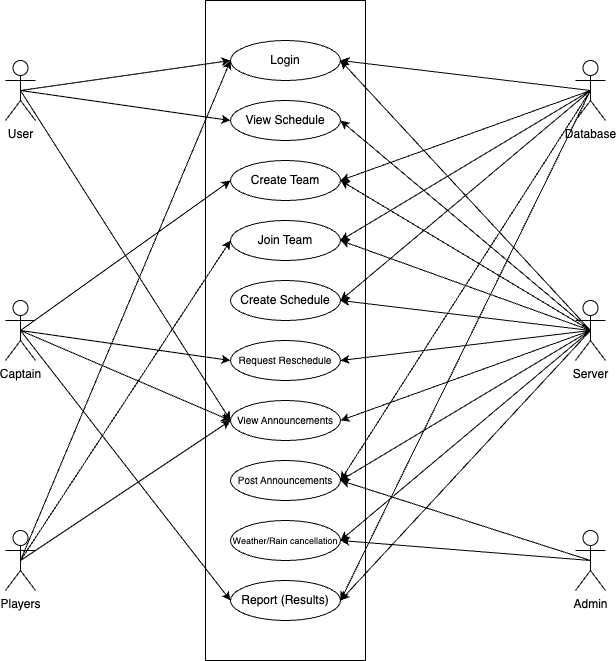
\includegraphics[width=\linewidth]{Use_case.png}
    \caption{Use Case Diagram}
    \label{fig:use_case}
\end{figure}
\pagebreak
\subsection{Individual Product Use Cases (PUC's)}
\begin{itemize}
\item \textbf{UC1:} Login \\
	Trigger: User enters their username and password.\\
	Preconditions: Client is not logged in to the system with an existing account.\\
	Actors: User, Captain, Player, Database, Server.\\
	Outcome: If the username and password is a match with an account in
	the database, the user is logged in. If not, then the user is prompted
	to try again, reset password (if username exists) or create an account.
\item \textbf{UC2:} View Schedule \\
	Trigger: User interacts with the view schedule prompt.\\
	Preconditions: N/A (All users can view schedule)\\
	Actors: User, Database, Server
	Outcome: Page opens up with the schedule for the GSA softball league season.
\item \textbf{UC3:} View Standings \\
	Trigger: User interacts with View standings prompt.\\
	Preconditions: N/A (All users can view standings)\\
	Actors: User, Database, Server.\\
	Outcome: The standings for the GSA softball league season is displayed.
\item \textbf{UC4:} Create Team \\
	Trigger: User request to make a team with team info.\\
	Preconditions: Client is logged in to the system as a Captain.\\
	Actors: User, Captain, Database, Server.\\
	Outcome: If the team name is unique and the user is not already an existing member
	of another team, the team is created with the user as the Captain of the team.
\item \textbf{UC5:} Join Team \\
	Trigger: User request to join an already existing team\\
	Preconditions: User is logged into the system, the user is not part of an
	already existing team, and team being requested exists.\\
	Actors: User, Player, Database, Server.\\
	Outcome: If the user is logged in and is not a member of an already existing team, then
	the user will receive a request to fill out the waiver if the team exists. Upon completion,
	the user becomes a member of that team.
\item \textbf{UC6:} Create Schedule \\
	Trigger: Registration deadline is past due.\\
	Preconditions: Teams are registered in the league and meet the team conditions.\\
	Actors: Server.\\
	Outcome: The system uses the team preferences and creates a schedule with all open slots.
\item \textbf{UC7:} Request Reschedule \\
	Trigger: Captain interacts with the reschedule prompt at least 24 hours before the start time.\\
	Preconditions: Team exists and has a scheduled game.\\
	Actors: User, Captain, Database, Server.\\
	Outcome: If the user is a Captain and makes a request on an existing game at least 24 hours before
	the start, the Captain is able to view available slots for the game. Upon choosing an empty slot, the
	game schedule is updated.
\item \textbf{UC8:} View Announcements \\
	Trigger: User interacts with view announcement prompt.\\
	Preconditions: N/A (All users can view announcements).\\
	Actors: User, Captain, Player, Database, Server.\\
	Outcome: The announcements for the GSA softball league season is displayed.
\item \textbf{UC9:} Post Announcements \\
	Trigger: User interacts with the post announcement prompt.\\
	Preconditions: User must me logged in as an Admin.\\
	Actors: User, Admin, Database, Server.\\
	Outcome: If the user is logged in as an admin, and enters all the necessary information to complete
	the required sections for the announcements, the announcements is created and published on the GSA
	softball league platform.
\item \textbf{UC10:} Rain Cancellation/Override \\
	Trigger: User interacts with the Override prompt.\\
	Preconditions: User must me logged in as an Admin.\\
	Actors: User, Admin, Database, Server.\\
	Outcome: If the user is logged in as an admin, the user is able to cancel games or move then to open
	slots. Upon completion, the schedule is updated.
\item \textbf{UC11:} Report Results \\
	Trigger: User interacts with the report prompt.\\
	Preconditions: The user must be logged in as a Captain and the duration of a game must be elapsed after
	the scheduled start time.\\
	Actors: User, Captain, Database, Server.\\
	Outcome: If the user is logged in as a captain, and the duration of a game has been elapsed since the 
	start time, then the Captain is able to update the status of the game with results. Upon completion 
	the standings and game results are updated on the system.
\end{itemize}


\section{Functional Requirements}
This section details the core functional requirements of the system, organized by feature area. Each requirement includes a unique identifier, description, rationale, and measurable fit criteria. Requirements are traced to their corresponding use cases and dependencies.

% Authentication Requirements
\textbf{Requirement ID:} FR1 \quad \textbf{Type:} Functional \quad \textbf{Use Case:} UC1 \\
\textbf{Priority:} High \\
\textbf{Description:} The platform shall provide a secure login system where users enter credentials (email, password) to access the system. The system must:
\begin{itemize}
    \item Validate user credentials against encrypted database records
    \item Lock accounts after \hyperref[MAX_LOGIN_ATTEMPTS]{\texttt{MAX\_LOGIN\_ATTEMPTS}} failed attempts
    \item Enforce password complexity requirements
\end{itemize}
\textbf{Rationale:} Ensures secure access to the platform and role-specific functionality.\\
\textbf{Fit Criterion:} 
\begin{itemize}
    \item Authentication responses within \hyperref[MAX_RESPONSE_TIME]{\texttt{MAX\_RESPONSE\_TIME}} second
    \item Zero unauthorized access incidents
    \item 100\% successful login rate for valid credentials
\end{itemize}
\textbf{Customer Satisfaction:} 5 \quad\quad \textbf{Customer Dissatisfaction:} 5 \\
\textbf{Dependencies:} Database system\\
\textbf{Conflicts:} None\\
\noindent\rule{\textwidth}{1pt}

% Role-Based Access
\textbf{Requirement ID:} FR2 \quad \textbf{Type:} Functional \quad \textbf{Use Case:} UC6, UC7, UC9, UC10, UC11 \\
\textbf{Priority:} High \\
\textbf{Description:} The platform shall implement role-based access control (RBAC) with distinct permissions for commissioners, captains, and players. The system must:
\begin{itemize}
    \item Enforce role-specific access restrictions
    \item Maintain audit logs of permission changes
    \item Support role assignment and modification
\end{itemize}
\textbf{Rationale:} Ensures appropriate access levels and maintains system security.\\
\textbf{Fit Criterion:} 
\begin{itemize}
    \item 100\% accurate role-based access enforcement
\end{itemize}
\textbf{Customer Satisfaction:} 5 \quad\quad \textbf{Customer Dissatisfaction:} 5 \\
\textbf{Dependencies:} FR1 (Authentication System)\\
\textbf{Conflicts:} None\\
\noindent\rule{\textwidth}{1pt}

\textbf{Requirement ID:} FR3 \quad \textbf{Type:} Functional \quad \textbf{Use Case:} UC2 \\
\textbf{Description:} The system shall provide three distinct schedule viewing options:
\begin{itemize}
    \item Weekly Team Schedule View:
    \begin{itemize}
        \item Display current week's games for user's team
        \item Show date, time, location, and opponent for each game
    \end{itemize}
    \item Monthly Team Schedule View:
    \begin{itemize}
        \item Calendar view of the month showing all of the user's team games
        \item Show date, time, location, and opponent for each game
        \item Allow users to navigate between different months
    \end{itemize}
    \item Monthly League Schedule View:
    \begin{itemize}
        \item Complete calendar of all league games
        \item Show date, time, location, and home/away teams for each game
        \item Allow users to navigate between different months
    \end{itemize}
\end{itemize}
\textbf{Rationale:} Multiple view options provide flexibility for different user needs and planning horizons while ensuring comprehensive schedule access.\\
\textbf{Fit Criterion:} 
\begin{itemize}
    \item All three views accurately display game information
    \item Users can seamlessly switch between views
    \item Calendar integration works with major calendar systems
    \item Views update within 5 seconds of schedule changes
    \item 100\% of scheduled games appear in appropriate views
\end{itemize}
\textbf{Customer Satisfaction:} 5 \quad\quad \textbf{Customer Dissatisfaction:} 5\\
\textbf{Dependencies:} Game scheduling system, user authentication\\
\textbf{Conflicts:} None\\
\noindent\rule{\textwidth}{1pt}

\textbf{Requirement ID:} FR4 \quad \textbf{Type:} Functional \quad \textbf{Use Case:} UC3 \\
\textbf{Description:} The platform shall provide an accurate display of league standings for all registered users.\\
\textbf{Rationale:} Keeps league members informed of team rankings.\\
\textbf{Fit Criterion:} League standings are updated accurately, automatically and visible to logged-in users.\\
\textbf{Customer Satisfaction:} 4 \quad\quad \textbf{Customer Dissatisfaction:} 4\\
\noindent\rule{\textwidth}{1pt}

\textbf{Requirement ID:} FR5 \quad \textbf{Type:} Functional \quad \textbf{Use Case:} UC4 \\
\textbf{Priority:} High \\
\textbf{Description:} The platform shall allow captains to create a team by entering team details and submitting for registration.\\
\textbf{Rationale:} Enables team formation and league participation.\\
\textbf{Fit Criterion:} Captains can create a team, and details are stored in the system.\\
\textbf{Customer Satisfaction:} 5 \quad\quad \textbf{Customer Dissatisfaction:} 5\\
\noindent\rule{\textwidth}{1pt}

\textbf{Requirement ID:} FR6 \quad \textbf{Type:} Functional \quad \textbf{Use Case:} UC5 \\
\textbf{Priority:} High \\
\textbf{Description:} The system shall provide team captains with the exclusive ability to invite players to their team. The invitation process must:
\begin{itemize}
    \item Allow captains to send invitations to players via email
    \item Allow invited players to accept or decline the invitation
    \item Automatically update team rosters upon invitation acceptance
\end{itemize}
\textbf{Rationale:} Centralizing team formation control with captains ensures organized roster management and clear accountability for team composition.\\
\textbf{Fit Criterion:} 
\begin{itemize}
    \item Only team captains can initiate player invitations
    \item Players cannot join teams without a captain's invitation
    \item System prevents duplicate invitations to the same player
    \item Players already on a team cannot be invited to another team
    \item 100\% of roster updates are accurately reflected after invitation acceptance
\end{itemize}
\textbf{Customer Satisfaction:} 4 \quad\quad \textbf{Customer Dissatisfaction:} 5\\
\textbf{Dependencies:} User authentication system, email notification system\\
\textbf{Conflicts:} None\\
\noindent\rule{\textwidth}{1pt}

\textbf{Requirement ID:} FR7 \quad \textbf{Type:} Functional \quad \textbf{Use Case:} UC6 \\
\textbf{Priority:} High \\
\textbf{Description:} The platform shall automatically generate the season game schedule based on team availability and preferences.\\
\textbf{Rationale:} Automates scheduling for league to begin with improved efficiency.\\
\textbf{Fit Criterion:} The system generates a schedule that gives all teams equal games and factors in team preferences.\\
\textbf{Customer Satisfaction:} 5 \quad\quad \textbf{Customer Dissatisfaction:} 5\\
\noindent\rule{\textwidth}{1pt}

\textbf{Requirement ID:} FR8 \quad \textbf{Type:} Functional \quad \textbf{Use Case:} UC7 \\
\textbf{Priority:} High \\
\textbf{Description:} The platform shall allow captains to request a reschedule by selecting a new time slots for an existing game.\\
\textbf{Rationale:} Enables flexibility and error-handling in scheduling.\\
\textbf{Fit Criterion:} Captains can successfully submit reschedule requests, and the system tracks pending requests.\\
\textbf{Customer Satisfaction:} 4 \quad\quad \textbf{Customer Dissatisfaction:} 5\\
\noindent\rule{\textwidth}{1pt}

\textbf{Requirement ID:} FR9 \quad \textbf{Type:} Functional \quad \textbf{Use Case:} UC8 \\
\textbf{Priority:} Medium \\
\textbf{Description:} The platform shall allow users to view league-wide announcements, lost and found, weather updates on the dashboard.\\
\textbf{Rationale:} Keeps users informed about important league updates. \\
\textbf{Fit Criterion:} Announcements are displayed in the users announncement dashboard.\\
\textbf{Customer Satisfaction:} 4 \quad\quad \textbf{Customer Dissatisfaction:} 3\\
\noindent\rule{\textwidth}{1pt}

\textbf{Requirement ID:} FR10 \quad \textbf{Type:} Functional \quad \textbf{Use Case:} UC9 \\
\textbf{Priority:} Medium \\
\textbf{Description:} The platform shall allow administrators to post announcements that are visible to all users.\\
\textbf{Rationale:} Enables effective communication with all participants.\\
\textbf{Fit Criterion:} Administrators can post announcements to be viewable by players.\\
\textbf{Customer Satisfaction:} 3 \quad\quad \textbf{Customer Dissatisfaction:} 3\\
\noindent\rule{\textwidth}{1pt}

\textbf{Requirement ID:} FR11 \quad \textbf{Type:} Functional \quad \textbf{Use Case:} UC10 \\
\textbf{Priority:} High \\
\textbf{Description:} The platform shall allow administrators to manually cancel or reschedule games due to weather conditions or accepted requests.\\
\textbf{Rationale:} Ensures timely communication for game rescheduling or cancellations.\\
\textbf{Fit Criterion:} Administrators can cancel or reschedule games, which updates the schedule, and teams are notified automatically. \\
\textbf{Customer Satisfaction:} 5 \quad\quad \textbf{Customer Dissatisfaction:} 4\\
\noindent\rule{\textwidth}{1pt}

\textbf{Requirement ID:} FR12 \quad \textbf{Type:} Functional \quad \textbf{Use Case:} UC11 \\
\textbf{Priority:} High \\
\textbf{Description:} The platform shall allow captains to report game scores and forfeits by selecting a completed game and submitting the final result.\\
\textbf{Rationale:} Simplifies reporting and keeps standings up to date.\\
\textbf{Fit Criterion:} Captains can submit game results, and standings are updated automatically. \\
\textbf{Customer Satisfaction:} 4 \quad\quad \textbf{Customer Dissatisfaction:} 3\\
\noindent\rule{\textwidth}{1pt}

\textbf{Requirement ID:} FR13 \quad \textbf{Type:} Functional \quad \textbf{Use Case:} UC8 \\
\textbf{Priority:} High \\
\textbf{Description:} The system shall provide a player profile management interface that allows users to:
\begin{itemize}
    \item View and update personal information:
    \begin{itemize}
        \item First name and last name
        \item Email address
        \item Phone number
    \end{itemize}
\end{itemize}
\textbf{Rationale:} Centralized profile management ensures accurate player information for league communications and emergency situations.\\
\textbf{Fit Criterion:} 
\begin{itemize}
    \item All profile updates are saved and reflected immediately
    \item Email addresses are validated for correct format
    \item Phone numbers are validated for correct format
    \item Changes are logged for audit purposes
\end{itemize}
\textbf{Customer Satisfaction:} 4 \quad\quad \textbf{Customer Dissatisfaction:} 4\\
\textbf{Dependencies:} User authentication system, data encryption system\\
\textbf{Conflicts:} None\\
\noindent\rule{\textwidth}{1pt}

\section{Non-Functional Requirements}
The following requirements labeled with [HA] are derived from the Hazard Analysis document.

\subsection{Data Integrity and Backup Requirements}
\textbf{Requirement ID:} NFR7 [HA4] \quad \textbf{Type:} Non-Functional \\
\textbf{Priority:} Must Have \\
\textbf{Description:} The platform shall implement comprehensive data integrity and backup mechanisms:
\begin{itemize}
    \item Schedule and perform regular data backups and integrity checks
    \item Backup all critical data (game results, standings, user profiles) daily during season
    \item Store backups in geographically separate location for security
    \item Enable data restoration from latest backup
    \item Test backup and recovery processes each season
\end{itemize}
\textbf{Rationale:} Guarantee that the platform can recover from any potential data loss or corruption.\\
\textbf{Fit Criterion:} 
\begin{itemize}
    \item 100\% successful backup verification and restore testing
    \item Data backups must occur at least once daily during the season
    \item Backup and recovery processes must be tested every season
\end{itemize}
\textbf{Dependencies:} Database system\\
\textbf{Conflicts:} None\\

\subsection{Session Management Requirements}
\textbf{Requirement ID:} NFR8 [HA5] \quad \textbf{Type:} Non-Functional \\
\textbf{Priority:} Must Have \\
\textbf{Description:} The platform shall implement robust session management:
\begin{itemize}
    \item Automatic session timeouts after 10 minutes of inactivity
    \item Display countdown warning 1 minute before timeout
    \item Require re-authentication after timeout
\end{itemize}
\textbf{Rationale:} Prevent unauthorized access on shared devices and enhance security.\\
\textbf{Fit Criterion:} 
\begin{itemize}
    \item All inactive sessions must terminate within specified timeframe
    \item 100\% of timeouts must trigger re-authentication
\end{itemize}
\textbf{Dependencies:} Authentication system\\
\textbf{Conflicts:} None\\

\subsection{Audit Logging Requirements}
\textbf{Requirement ID:} NFR9 [HA6] \quad \textbf{Type:} Non-Functional \\
\textbf{Priority:} Should Have \\
\textbf{Description:} The platform shall implement comprehensive audit logging:
\begin{itemize}
    \item Log all critical actions (logins, schedule changes, roster updates)
    \item Store logs securely with encryption
    \item Retain logs for minimum 90 days
    \item Enable admin search and filtering of logs
    \item Generate real-time alerts for suspicious activities
\end{itemize}
\textbf{Rationale:} Enable troubleshooting and security monitoring.\\
\textbf{Fit Criterion:} 
\begin{itemize}
    \item 100\% logging coverage of critical actions
    \item Logs must be retained for minimum 90 days
    \item Real-time alert generation for suspicious activities
\end{itemize}
\textbf{Dependencies:} Storage system, encryption system\\
\textbf{Conflicts:} None\\

\subsection{Security Testing Requirements}
\textbf{Requirement ID:} NFR10 [HA7] \quad \textbf{Type:} Non-Functional \\
\textbf{Priority:} Must Have \\
\textbf{Description:} The platform shall undergo comprehensive security testing:
\begin{itemize}
    \item Perform end-to-end security testing
    \item Automate security tests for consistent application
    \item Test for common vulnerabilities (SQL injection, XSS)
\end{itemize}
\textbf{Rationale:} Ensure platform security against potential threats.\\
\textbf{Fit Criterion:} 
\begin{itemize}
    \item All security tests must pass before deployment
    \item Zero known security vulnerabilities in production
\end{itemize}
\textbf{Dependencies:} Testing framework\\
\textbf{Conflicts:} None\\

\subsection{Schedule Verification Requirements}
\textbf{Requirement ID:} NFR11 [HA8] \quad \textbf{Type:} Non-Functional \\
\textbf{Priority:} Must Have \\
\textbf{Description:} The platform shall implement automated schedule verification:
\begin{itemize}
    \item Verify schedule completeness automatically
    \item Check for missing games or conflicts
    \item Validate fair distribution of games
\end{itemize}
\textbf{Rationale:} Prevent scheduling errors and ensure fairness in game distribution.\\
\textbf{Fit Criterion:} 
\begin{itemize}
    \item Zero undetected scheduling conflicts
    \item Zero missing games in generated schedules
    \item Equal game distribution among teams
\end{itemize}
\textbf{Dependencies:} Scheduling system\\
\textbf{Conflicts:} None\\

\section{Look and Feel Requirements}
This section details the non-functional requirements for the look and feel of the platform.
\subsection{Layout Requirements}
\textbf{Requirement ID:} NFR-LF3 \quad \textbf{Type:} Non-Functional \\
\textbf{Description:} The platform shall maintain a responsive layout that adapts to different screen sizes and devices, ensuring optimal viewing and interaction across desktop and mobile platforms.\\
\textbf{Fit Criterion:} The interface must maintain usability and readability across all common device sizes (mobile, tablet, desktop) with no horizontal scrolling required.

\subsection{Visual Feedback Requirements}
\textbf{Requirement ID:} NFR-LF4 \quad \textbf{Type:} Non-Functional \\
\textbf{Description:} The platform shall provide clear visual feedback for all user actions, including loading states, success/error messages, and interactive element states.\\
\textbf{Fit Criterion:} All user actions must receive immediate visual feedback, and system status changes must be clearly indicated to users.


\subsection{Appearance Requirements}
\textbf{Requirement ID:} NFR-LF1 \quad \textbf{Type:} Non-Functional \\
\textbf{Description:} The platform must feature a modern, intuitive interface with consistent visual elements across all views to ensure ease of use.\\
\textbf{Fit Criterion:} \hyperref[USER_INTERFACE_RATING]{\texttt{USER\_INTERFACE\_RATING}}\% of users should rate the interface as "intuitive" or "very intuitive" in usability surveys.

\subsection{Style Requirements}
\textbf{Requirement ID:} NFR-LF2 \quad \textbf{Type:} Non-Functional \\
\textbf{Description:} The platform shall follow a consistent color palette, typography, and layout to ensure ease of use, and improve accessibility by maintaining predictable design elements across the platform.\\
\textbf{Fit Criterion:} All pages must use the defined style guide elements with 100\% compliance.

\section{Usability and Humanity Requirements}
\subsection{Ease of Use Requirements}
\textbf{Requirement ID:} NFR-U1 \quad \textbf{Type:} Non-Functional \\
\textbf{Description:} Graduate students and other users shall be able to complete common tasks (login, team creation, schedule viewing) within an average of 3 minutes with no prior experience or external help.\\
\textbf{Fit Criterion:} \hyperref[TASK_COMPLETION_RATE]{\texttt{TASK\_COMPLETION\_RATE}}\% of new users should complete basic tasks within the specified time frame.

\subsection{Personalization and Internationalization Requirements}
\textbf{Requirement ID:} NFR-U2 \quad \textbf{Type:} Non-Functional \\
\textbf{Description:} The platform must be tailored to Canadian English, using the metric system for measurements and adhering to local date and time formats.\\
\textbf{Fit Criterion:} 100\% compliance with Canadian date/time formats and measurement standards.

\subsection{Learning Requirements}
\textbf{Requirement ID:} NFR-U3 \quad \textbf{Type:} Non-Functional \\
\textbf{Description:} The platform must provide clear instructions and tooltips on all views to help new users quickly learn how to navigate and use key features.\\
\textbf{Fit Criterion:} \hyperref[LEARNING_SUCCESS_RATE]{\texttt{LEARNING\_SUCCESS\_RATE}}\% of new users should be able to complete basic tasks without requiring support.

\subsection{Understandability and Politeness Requirements}
\textbf{Requirement ID:} NFR-U4 \quad \textbf{Type:} Non-Functional \\
\textbf{Description:} The platform must provide clear, straightforward navigation with simply labeled menus and buttons so that minimal prior knowledge is required.\\
\textbf{Fit Criterion:} All navigation elements must have clear, descriptive labels with no technical jargon.

\subsection{Accessibility Requirements}
\textbf{Requirement ID:} NFR-U5 \quad \textbf{Type:} Non-Functional \\
\textbf{Description:} The platform shall provide basic accessibility features, such as keyboard navigation and sufficient text contrast, to ensure usability for a wide range of users.\\
\textbf{Fit Criterion:} Meet WCAG 2.1 Level AA compliance requirements.

\section{Performance Requirements}
\subsection{Speed and Latency Requirements}
\textbf{Requirement ID:} NFR-P1 \quad \textbf{Type:} Non-Functional \\
\textbf{Description:} The platform must respond to user actions (e.g., scheduling, score reporting) within \hyperref[MAX_RESPONSE_TIME]{\texttt{MAX\_RESPONSE\_TIME}} second to contribute to user satisfaction and efficiency.\\
\textbf{Fit Criterion:} \hyperref[ACTION_COMPLETION_RATE]{\texttt{ACTION\_COMPLETION\_RATE}}\% of all user actions must complete within the specified time limit.

\subsection{Safety-Critical Requirements}
\textbf{Requirement ID:} NFR-P2 \quad \textbf{Type:} Non-Functional \\
\textbf{Description:} The platform must ensure the secure and accurate storage of player personal information and waivers, preventing data loss or corruption.\\
\textbf{Fit Criterion:} Zero instances of data loss or unauthorized access.

\subsection{Precision or Accuracy Requirements}
\textbf{Requirement ID:} NFR-P3 \quad \textbf{Type:} Non-Functional \\
\textbf{Description:} The platform must calculate and display the standings with 100\% accuracy and accurately match game preferences with available slots to avoid conflicts.\\
\textbf{Fit Criterion:} 100\% accuracy in standings calculations and zero scheduling conflicts.

\subsection{Robustness or Fault-Tolerance Requirements}
\textbf{Requirement ID:} NFR-P4 \quad \textbf{Type:} Non-Functional \\
\textbf{Description:} The platform shall handle failed database connections by logging the error and displaying an error message to the user, and allow users to retry their actions.\\
\textbf{Fit Criterion:} All system errors must be logged and users must be able to retry failed actions.

\subsection{Capacity Requirements}
\textbf{Requirement ID:} NFR-P5 \quad \textbf{Type:} Non-Functional \\
\textbf{Description:} The platform must be able to store and handle the scheduling for at minimum \hyperref[MAX_TEAM_CAPACITY]{\texttt{MAX\_TEAM\_CAPACITY}} teams in the league to ensure scheduling handling and league expansion.\\
\textbf{Fit Criterion:} Successfully manage \hyperref[MAX_TEAM_CAPACITY]{\texttt{MAX\_TEAM\_CAPACITY}} teams with no degradation in performance.

\subsection{Scalability or Extensibility Requirements}
\textbf{Requirement ID:} NFR-P6 \quad \textbf{Type:} Non-Functional \\
\textbf{Description:} The platform shall support handling up to \hyperref[MAX_TEAM_CAPACITY]{\texttt{MAX\_TEAM\_CAPACITY}} teams without performance issues to ensure scheduling handling and website performance for a full league.\\
\textbf{Fit Criterion:} System performance must remain consistent when managing \hyperref[MAX_TEAM_CAPACITY]{\texttt{MAX\_TEAM\_CAPACITY}} teams.

\subsection{Longevity Requirements}
\textbf{Requirement ID:} NFR-P7 \quad \textbf{Type:} Non-Functional \\
\textbf{Description:} The platform must use modern, widely supported web technologies to ensure long-term compatibility with future devices and browsers.\\
\textbf{Fit Criterion:} Compatible with all major browsers and devices for at least \hyperref[BROWSER_COMPATIBILITY_YEARS]{\texttt{BROWSER\_COMPATIBILITY\_YEARS}} years.

\section{Operational and Environmental Requirements}
\subsection{Expected Physical Environment}
\textbf{Requirement ID:} NFR-O1 \quad \textbf{Type:} Non-Functional \\
\textbf{Description:} The platform must be accessible on various devices, such as desktops, laptops, smartphones, and tablets, with a stable internet connection and appropriate server infrastructure.\\
\textbf{Fit Criterion:} 100\% functionality across all specified device types.

\subsection{Browser Compatibility}
\textbf{Requirement ID:} NFR-O2 \quad \textbf{Type:} Non-Functional \\
\textbf{Description:} The platform must be accessible across multiple browsers with responsive design that allows users to reach all features when using a mobile device.\\
\textbf{Fit Criterion:} Full functionality in Chrome, Safari, Firefox, and Edge browsers.

\subsection{Requirements for Interfacing with Adjacent Systems}
\textbf{Requirement ID:} NFR-O3 \quad \textbf{Type:} Non-Functional \\
\textbf{Description:} The platform must support integration with payment gateways, calendar systems, and data import/export functionality for roster data and match results.\\
\textbf{Fit Criterion:} Successful integration with specified external systems with \hyperref[SYSTEM_UPTIME]{\texttt{SYSTEM\_UPTIME}}\% uptime.

\subsection{Productization Requirements}
\textbf{Requirement ID:} NFR-O4 \quad \textbf{Type:} Non-Functional \\
\textbf{Description:} The platform must handle scaling well, such as an increased number of divisions, teams, players, etc. League managers should be able to manage game rules and related information.\\
\textbf{Fit Criterion:} System maintains performance with up to \hyperref[MAX_TEAMS]{\texttt{MAX\_TEAMS}} teams and supports rule management within \hyperref[ADMIN_CHANGE_TIME]{\texttt{ADMIN\_CHANGE\_TIME}} minutes.

\subsection{Release Requirements}
\textbf{Requirement ID:} NFR-O5 \quad \textbf{Type:} Non-Functional \\
\textbf{Description:} Version control is required for tracking changes and rollback capabilities. All production releases must undergo thorough testing with real users.\\
\textbf{Fit Criterion:} 100\% of changes tracked in version control and all releases tested with minimum \hyperref[MIN_TEST_USERS]{\texttt{MIN\_TEST\_USERS}} real users.

\section{Maintainability and Support Requirements}
\subsection{Maintenance Requirements}
\textbf{Requirement ID:} NFR-M1 \quad \textbf{Type:} Non-Functional \\
\textbf{Description:} The platform should be updated regularly for fixing bugs, adding new features, and security patches.\\
\textbf{Fit Criterion:} Monthly maintenance updates with zero critical bugs pending for more than \hyperref[MAINTENANCE_BUG_DAYS]{\texttt{MAINTENANCE\_BUG\_DAYS}} days.

\subsection{Supportability Requirements}
\textbf{Requirement ID:} NFR-M2 \quad \textbf{Type:} Non-Functional \\
\textbf{Description:} Any user who requires support should be directed to an email that handles issues with the platform.\\
\textbf{Fit Criterion:} Support requests acknowledged within \hyperref[SUPPORT_RESPONSE_HOURS]{\texttt{SUPPORT\_RESPONSE\_HOURS}} hours and resolved within \hyperref[SUPPORT_RESOLUTION_HOURS]{\texttt{SUPPORT\_RESOLUTION\_HOURS}} hours.

\subsection{Adaptability Requirements}
\textbf{Requirement ID:} NFR-M3 \quad \textbf{Type:} Non-Functional \\
\textbf{Description:} An admin user should be able to change game rules within \hyperref[ADMIN_CHANGE_TIME]{\texttt{ADMIN\_CHANGE\_TIME}} minutes, such as swapping a team's game schedule with another if needed.\\
\textbf{Fit Criterion:} \hyperref[ADMIN_CHANGE_SUCCESS]{\texttt{ADMIN\_CHANGE\_SUCCESS}}\% of administrative changes completed within specified time frame.

\section{Security Requirements}
\subsection{Access Requirements}
\textbf{Requirement ID:} NFR-S1 \quad \textbf{Type:} Non-Functional \\
\textbf{Description:} The platform must implement role-based access control with distinct permissions for administrators, team managers, and players.\\
\textbf{Fit Criterion:} Zero unauthorized access incidents and 100\% correct permission enforcement.

\subsection{Integrity Requirements}
\textbf{Requirement ID:} NFR-S3 \quad \textbf{Type:} Non-Functional \\
\textbf{Description:} All data entered such as team rosters, game schedules, and scores must be validated for accuracy and completeness.\\
\textbf{Fit Criterion:} 100\% validation of all data entries with error logging.

\subsection{Privacy Requirements}
Personal user data such as emails, phone numbers, etc., should be protected by encryption.

\subsection{Audit Requirements}
\textbf{Requirement ID:} NFR-S4 \quad \textbf{Type:} Non-Functional \\
\textbf{Description:} Logs of team history, game scores, roster updates, and game scheduling, should all be kept in case we ever need them to solve disputes.\\
\textbf{Fit Criterion:} Complete audit trail for all system changes maintained for 1 year.

\subsection{Immunity Requirements}
\textbf{Requirement ID:} NFR-S5 \quad \textbf{Type:} Non-Functional \\
\textbf{Description:} The platform should be protected against malicious web attacks.\\
\textbf{Fit Criterion:} Zero successful security breaches and 100\% compliance with OWASP security standards.

\section{Cultural Requirements}
\subsection{Cultural Requirements}
\textbf{Requirement ID:} NFR-C1 \quad \textbf{Type:} Non-Functional \\
\textbf{Description:} The platform should support multiple languages so that the diverse league participants can switch to their preferred language. The platform should only display the local time of Hamilton, as it is assumed that all league participants are in the same region where the games are being hosted.\\
\textbf{Fit Criterion:} Support for English and French languages with 100\% accurate time zone display.

\section{Compliance Requirements}
\subsection{Legal Requirements}
\textbf{Requirement ID:} NFR-L1 \quad \textbf{Type:} Non-Functional \\
\textbf{Description:} Users who no longer want to be part of the league should be able to delete their data. The platform must accommodate for this within 2 minutes.\\
\textbf{Fit Criterion:} 100\% of data deletion requests completed within specified timeframe.

\subsection{Standards Compliance Requirements}
\textbf{Requirement ID:} NFR-ST1 \quad \textbf{Type:} Non-Functional \\
\textbf{Description:} The platform must adhere to the following standards and regulations:
\begin{itemize}
    \item \textbf{Privacy Standards:}
    \begin{itemize}
        \item Personal Information Protection and Electronic Documents Act (PIPEDA) \cite{pipeda2023}
        \item Freedom of Information and Protection of Privacy Act (FIPPA) \cite{fippa2023}
        \item General Data Protection Regulation (GDPR) compliance for international users \cite{gdpr2023}
    \end{itemize}

    \item \textbf{Web Accessibility Standards:}
    \begin{itemize}
        \item Web Content Accessibility Guidelines (WCAG) 2.1 Level AA compliance \cite{wcag2023}
        \item Section 508 of the Rehabilitation Act \cite{section5082023}
    \end{itemize}

    \item \textbf{Sports League Standards:}
    \begin{itemize}
        \item Canadian Interuniversity Sport (CIS) guidelines for recreational sports \cite{cis2023}
        \item McMaster University Athletics and Recreation policies \cite{mcmaster2023}
    \end{itemize}

    \item \textbf{Technical Standards:}
    \begin{itemize}
        \item OWASP Top 10 Security Standards \cite{owasp2023}
        \item ISO/IEC 27001 Information Security Management \cite{iso27001}
        \item REST API Design Standards \cite{rest2023}
    \end{itemize}
\end{itemize}
\textbf{Fit Criterion:} 100\% compliance with all specified standards and regulations.

\subsection{Industry Best Practices}
\textbf{Requirement ID:} NFR-ST2 \quad \textbf{Type:} Non-Functional \\
\textbf{Description:} The platform will implement the following industry best practices:
\begin{itemize}
    \item \textbf{Data Management:}
    \begin{itemize}
        \item Regular data backups every \hyperref[DATA_BACKUP_FREQUENCY_DAYS]{\texttt{DATA\_BACKUP\_FREQUENCY\_DAYS}} days
        \item Data encryption at rest and in transit
        \item Secure password hashing using industry-standard algorithms
    \end{itemize}

    \item \textbf{User Experience:}
    \begin{itemize}
        \item Responsive design principles
        \item Mobile-first approach
        \item Consistent navigation patterns
        \item Page load time under \hyperref[PAGE_LOAD_TIME_SECONDS]{\texttt{PAGE\_LOAD\_TIME\_SECONDS}} seconds
        \item Database query response time under \hyperref[DATABASE_QUERY_TIME_MS]{\texttt{DATABASE\_QUERY\_TIME\_MS}} milliseconds
    \end{itemize}

    \item \textbf{Performance:}
    \begin{itemize}
        \item Database query optimization with response time under \hyperref[DATABASE_QUERY_TIME_MS]{\texttt{DATABASE\_QUERY\_TIME\_MS}}ms
        \item Regular performance monitoring and optimization
    \end{itemize}
\end{itemize}
\textbf{Fit Criterion:} All specified best practices must be implemented and verified through testing.

\section{Open Issues}
This section details the open issues that are still under discussion.
\begin{itemize}
    \item \textbf{User Interface Design}: Some aspects of the user interface are yet to be fully defined. Specific visual elements and interaction flows will be determined in collaboration with stakeholders during the design phase.
    \item \textbf{User Interface Testing}: Details on the testing methodology for the user interface are still under discussion. The testing plan will include usability testing with users from the target audience to ensure ease of use.
    \item \textbf{User Payment Tracking Feature}: The implementation specifics for the payment tracking feature for staff are still being finalized. Considerations are being made regarding how the status of each player's payment will be updated and stored.
    \item \textbf{Integration of Existing Features}: There are open questions regarding the best approach to integrate and improve existing features from the current website in the new platform.
\end{itemize}

\section{Off-the-Shelf Solutions}
This section details the off-the-shelf solutions that will be used in the project.
\subsection{Ready-Made Products}
There are no ready-made products that will be a part of our solution. The objective is to update and completely redesign the current softball league web-based platform. While features from the original platform will be transferred over to maintain continuity, the entire solution will be developed in-house based on updated requirements and best practices.

\subsection{Reusable Components}
While no third-party reusable components will be integrated, several features from the original platform, such as user authentication, team management, and scheduling, will be carried over to ensure continuity. These components will be updated and enhanced as part of the complete redesign to meet the new requirements.

\subsection{Products That Can Be Copied}
There are no external products that will be directly copied for this project. However, the redesign will reference the design and functional elements of the current website to maintain familiarity for existing users. Additionally, best practices from similar platforms will be researched and adapted to improve the user experience.


\section{New Problems}
This section details the new problems that may arise during the project.
\subsection{Effects on the Current Environment}
Implementing the new system will require a complete overhaul of the existing McMaster GSA softball league platform, which may cause temporary disruption to ongoing league activities. The outdated system will be replaced, and users accustomed to the old methods may face a learning curve during the transition. Additionally, migrating any existing data (such as player information, schedules, and standings) to the new platform will need to be handled carefully to avoid loss or corruption. However, the improved system will provide long-term benefits by reducing maintenance and manual input required by the commissioners and administrators. 
\subsection{Effects on the Installed Systems}
Since the current system is outdated integrating the new platform may require adjustments to the existing server infrastructure or cloud services. The new system will be built on modern technologies which may require updating the server environment to ensure compatibility with these technologies. If hosted on legacy systems, a migration to a cloud or updated hosting service might be required.
\subsection{Potential User Problems}
Users (commissioners, captains, players) who are familiar with the current platform may struggle with adapting to the new interface and features. Particularly, older users or users with less technical proficiency may have difficulty navigating the system or understanding new functionalities like the rescheduling workflow, leaderboard tracking, or player management. Proper documentation and user training will be necessary to ensure a smooth transition and reduce user frustration. Moreover, captains and commissioners may need additional guidance on using automated features like team creation, player approvals, and schedule rescheduling.
\subsection{Limitations in the Anticipated Implementation Environment That May
Inhibit the New Product}
The project must be compatible with various devices (desktop, tablet, mobile), which presents challenges in ensuring consistent performance and user experience across different screen sizes and browsers. Another potential limitation is the anticipated usage spikes, such as the heavy volume of rescheduling requests at the beginning of the season, which could strain the system. The hosting environment needs to handle potential scalability issues, and the system should be optimized for responsiveness during high-demand periods. There may also be limitations in integrating certain external services, such as payment verification systems, if APIs or infrastructure constraints arise.
\subsection{Follow-Up Problems}
After the initial launch of the new platform, follow-up issues may include bug fixes, additional feature requests, and ongoing user feedback that necessitates adjustments. Since the system will rely on certain automated processes (e.g., scheduling, score reporting), there may be edge cases or scenarios not accounted for during development, which would require post-launch refinements. Maintenance and updates to the platform will need to be addressed continuously to ensure smooth functionality, especially in response to league changes or growing participation numbers. Moreover, as the system expands, additional support or enhancements might be required to maintain security and efficiency.

\section{Tasks}
This section details the tasks that will be undertaken during the project.

\subsection{Project Planning}
The platform's development will follow a structured plan prioritizing the requirements as outlined in the SRS. The functional requirements have been grouped based on priority, with each group indicating the relevant requirement numbers. Non-functional requirements, such as look and feel, usability, and accessibility, will be applied throughout the project to ensure consistency across all phases.

\textbf{High Priority} – These features are critical for the functioning of the platform:
\begin{itemize}
    \item \textbf{User Authentication and Account Management} (Requirements FR1, FR2): Secure login and user roles (commissioner, captain, player).
    \item \textbf{Team Management} (Requirements FR5, FR6): Captains create teams, select divisions, and manage rosters. Players can request to join teams.
    \item \textbf{Schedule Generation} (Requirement FR7): Automatically generate schedules, ensuring even distribution and honoring team preferences for dates/times.
    \item \textbf{Score Reporting} (Requirements FR11, FR12): Captains report game scores and forfeits, updating standings automatically.
    \item \textbf{Rescheduling System} (Requirements FR8, FR11): Allow captains to reschedule games, with requests approved by commissioners. Handle conflict checks and queues for multiple requests.
\end{itemize}

\textbf{Medium Priority} – These features enhance the user experience but are not critical to the platform's core functionality:
\begin{itemize}
    \item \textbf{Player Login and Team Requests} (Requirement FR6): Players can log in, view team information, and request to join teams.
    \item \textbf{Rescheduling Queue Management} (Requirement FR8): Manage multiple rescheduling requests and enforce time restrictions (e.g., within 24 hours of a game).
    \item \textbf{Announcements} (Requirements FR9, FR10): Commissioners post league-wide announcements for all users.
\end{itemize}

\textbf{Low Priority} – Features that are "nice to have" but not necessary for platform operation:
\begin{itemize}
    \item \textbf{UI/UX Enhancements} (Non-functional requirement): A modern interface, cleaner design, weekly schedule tabs, and alternating colors for easier reading.
    \item \textbf{Lost and Found Feature} (Non-functional requirement): Allow users to report and check lost items.
    \item \textbf{Waiver System} (Non-functional requirement): Integrate waivers with payment status tracking.
\end{itemize}

\subsection{Planning of the Development Phases}
Development will be divided into phases, with each phase focused on implementing the functional requirements in order of priority. Each phase includes start and end dates based on your project schedule:

\subsubsection{Phase 1: Requirement Gathering and Initial Planning}
\textit{Start: September 10, 2024 | End: October 9, 2024}
\begin{itemize}
    \item Meet with stakeholders to determine the functional and non-functional requirements of the platform.
    \item Prioritize requirements based on their criticality to the project.
    \item Document the initial project plan, setting up deadlines for each phase.
\end{itemize}

\subsubsection{Phase 2: Proof of Concept and Design}
\textit{Start: October 10, 2024 | End: November 22, 2024}
\begin{itemize}
    \item Develop and demonstrate a proof of concept for high-priority features, including user authentication, team management, and scheduling (Requirements \#1, \#2, \#5, \#7).
    \item Finalize the design document and refine it based on stakeholder feedback.
\end{itemize}

\subsubsection{Phase 3: Core Development}
\textit{Start: November 23, 2024 | End: January 15, 2025}
\begin{itemize}
    \item Implement high-priority features, including team management, scheduling, and score reporting (Requirements \#5, \#7, \#11, \#12).
    \item Begin the integration of features from the existing platform where applicable.
\end{itemize}

\subsubsection{Phase 4: Verification, Validation, and Revision}
\textit{Start: January 16, 2025 | End: March 7, 2025}
\begin{itemize}
    \item Test the platform against the documented requirements.
    \item Present the initial version (Revision 0) and gather feedback for improvement.
\end{itemize}

\subsubsection{Phase 5: Final Development and Demonstration}
\textit{Start: March 8, 2025 | End: March 30, 2025}
\begin{itemize}
    \item Finalize medium- and low-priority features, such as announcements and UI/UX improvements (Requirements \#9, \#10, non-functional requirements).
    \item Prepare for the final demonstration and present the platform.
\end{itemize}

\subsubsection{Phase 6: Documentation and Wrap-Up}
\textit{Start: April 1, 2025 | End: April 2, 2025}
\begin{itemize}
    \item Complete all project documentation.
    \item Submit the final deliverables, including the user guide and source code.
\end{itemize}


\section{Migration to the New Product}
This section details the requirements for migrating to the new product.
\subsection{Requirements for Migration to the New Product}
To migrate from the existing platform to our redesign involves several key steps to ensure that the transfer of all relevant data, features, and functionalities is seamless and complete:

\begin{itemize}
    \item \textbf{Data Preservation}: All current data from the existing platform must be preserved and migrated to the new platform. The specific data to be transferred will be confirmed through consultation with the current platform administrator, ensuring that only the necessary and relevant data is included in the migration.
    \item \textbf{Feature Continuity}: Ensure that all features present in the original platform are retained in the redesigned version, with enhancements and improvements where applicable.
    \item \textbf{Minimizing Downtime}: The softball season begins in April, which falls around when the project is expected to be completed. Due to this tight deadline, the migration process should be planned to minimize downtime for users, ensuring that the transition is as smooth as possible with minimal impact on league operations.
\end{itemize}

\subsection{Data That Has to be Modified or Translated for the New System}
During the migration process, specific data elements may need to be modified or translated to align with the new platform's structure and data requirements:

\begin{itemize}
    \item \textbf{User Accounts and Roles}: The login system needs a complete redesign. User account information, including usernames, passwords, and roles (commissioner, captain, player), will need to be reformatted to match the requirements of the new authentication system.
    \item \textbf{Team and Match Data}: Team rosters, match schedules, and historical results may require adjustments to fit the new database schema. This may involve reformatting data fields or translating old data structures to new formats.
\end{itemize}

\section{Costs}
The capstone supervisor expressed minimizing costs. Our approach will be done with free frameworks, such as React.js, and affordable hosting plans such as AWS or Google Cloud. Our team will emphasize core functionality, and avoid creating unnecessary features and costs that could undermine the product goal. By following these cost-conscious strategies, the project can stay within budget while delivering a functional and scalable platform.

\section{User Documentation and Training}
This section details the user documentation and training requirements.
\subsection{User Documentation Requirements}
\begin{itemize}
    \item \textbf{Comprehensive User Guide}: Create a detailed user manual page tab that outlines:
    \begin{itemize}
        \item \textbf{Getting Started}: Instructions on how to register, create teams, and navigate the platform before delving deep into more advanced features.
        \item \textbf{Feature Descriptions}: Written and visual explanations of each feature, such as team management, scheduling, score tracking, etc.
        \item \textbf{FAQs}: Address common questions and troubleshooting tips to help users resolve issues independently. If unresolved, prompt users to email for more support or direct them to the discussions page.
    \end{itemize}
    \item \textbf{Interactive Tutorials}: Create pop-up icons that demonstrate key functionalities, making it easier for both new and existing users to understand how to use the platform effectively.
\end{itemize}

\subsection{Training Requirements}
\begin{itemize}
    \item \textbf{Help Support Desk}: A dedicated support email or live chat feature where users can ask questions or report issues with someone real.
    \item \textbf{Feedback Section}: Implement a section where users can provide feedback through open-ended surveys to help improve the platform.
    \item \textbf{Discussion}: A section where users can publicly post their questions and other users are free to answer them.
\end{itemize}

\section{Waiting Room}
For the softball league platform, the "waiting room" will most likely be the feature for players who have registered, but do not have a pre-formed team. These players are called "free agents," who may be added to teams later once all team rosters are confirmed. This concept is similar to how IMLeague is handled, which is the McMaster Intramural League platform. For example, a student desires to play softball and registers for the platform. As pre-formed teams are registered and confirmed, this student will be assigned to one of the teams that have extra space on their roster. Hence, they are "waiting" for a team to join.

\section{Ideas for Solution}
Players who sign up without a pre-formed team will be placed in a waiting room, designating them as "free agents." This waiting room is a holding area until all team rosters are confirmed. Other teams can choose from this holding area if they need any players before the final roster confirmation date. However, all players will eventually be auto-assigned to a team if the waiting room is still non-empty. Players from the waiting room will be notified of status updates. Players who register late will also be automatically assigned from the waiting room.

Therefore, we need a database to hold the status of each player in the waiting room. On the front user interface, the waiting room should be displayed to all users, so teams can see available free agents. For users with team manager permissions, they will be able to invite free agents from the waiting room to their teams if desired.


\newpage{}
\section*{Appendix --- Reflection}

The purpose of reflection questions is to give you a chance to assess your own
learning and that of your group as a whole, and to find ways to improve in the
future. Reflection is an important part of the learning process.  Reflection is
also an essential component of a successful software development process.  

Reflections are most interesting and useful when they're honest, even if the
stories they tell are imperfect. You will be marked based on your depth of
thought and analysis, and not based on the content of the reflections
themselves. Thus, for full marks we encourage you to answer openly and honestly
and to avoid simply writing ``what you think the evaluator wants to hear.''

Please answer the following questions.  Some questions can be answered on the
team level, but where appropriate, each team member should write their own
response:


\begin{enumerate}
    \item \textbf{What went well while writing this deliverable?}
    
    During the development of the SRS, the team was able to collaborate effectively, maintaining open communication and sharing ideas. The clear breakdown of tasks among team members helped streamline the process, ensuring that each section was tackled methodically. We used Google Docs to put down initial drafts and brainstorming so we could work together more easily in real time than if we were to draft using git commits. Utilizing LaTeX as the documentation format facilitated a consistent and professional layout, making it easy to organize and adjust content as needed.

    \item \textbf{What pain points did you experience during this deliverable, and how did you resolve them?}
    
    One of the major challenges faced was ensuring that all requirements were accurately captured and properly categorized, especially distinguishing between functional and non-functional requirements. To resolve this, team members would bring up to the rest of the team any concerns they had in their designated sections. Another key step was comparing the requirements document with feedback from the TA. Additionally, managing the document formatting in LaTeX was initially time-consuming, but the team grew more proficient over time through consistent practice and peer assistance. Another pain point would be the struggle to keep track of all graded content and requirements. This was because the resources we have disributed over GitLab, GitHub, and AvenueToLearn. This caused a lot of confusion for the team that we still need to get adapt to.

    \item \textbf{How many of your requirements were inspired by speaking to your client(s) or their proxies (e.g., your peers, stakeholders, potential users)?}
    
    A significant portion of the requirements—approximately 80\%—were directly inspired by interactions with the client (our project advisor). Discussion with the project advisor provided valuable insights, helping the team refine specific requirements related to user roles, scheduling, and data management.

    \item \textbf{Which of the courses you have taken, or are currently taking, will help your team to be successful with your capstone project?}
    
    The following courses are expected to be instrumental in the success of this project:
    \begin{itemize}
        \item \textbf{SFWRENG 4HC3 (Human-Computer Interfaces):} This course provides essential knowledge for designing user-friendly interfaces, critical for the web platform.
        \item \textbf{SFWRENG 4AA4 (Real-Time Systems and Control Applications):} Offers insights into designing responsive systems, which is important for building the scheduling and management components of the platform.
        \item \textbf{SFWRENG 3DB3 (Databases):} Provides the necessary skills for designing and managing databases, crucial for the project’s data management requirements.
        \item \textbf{SFWRENG 2C03 (Data Structures and Algorithms):} A foundational course that covers algorithms relevant to the scheduling functionality of the platform.
        \item \textbf{SFWRENG 3S03 (Software Testing \& Quality Assurance):} This course will aid in implementing rigorous testing methodologies to ensure that the platform meets the required quality standards.
    \end{itemize}
    
    \item \textbf{What knowledge and skills will the team collectively need to acquire to successfully complete this capstone project?} \\
    The team will need to acquire skills in several areas to ensure the successful development of the softball league platform. These include:
    \begin{itemize}
        \item \textbf{Front-End Development and User Interface Design:} Knowledge of creating user-friendly and accessible interfaces, applying Human-Computer Interfaces (HCI) principles.
        \item \textbf{Database Management:} Skills related to structuring, optimizing, and securing databases to handle large volumes of user data.
        \item \textbf{Scheduling Algorithms:} Familiarity with creating effective scheduling systems that allow team preferences and rescheduling requests to be efficiently managed.
        \item \textbf{Authentication and Security:} Understanding of secure login systems and data protection measures to ensure user information is kept safe.
        \item \textbf{System Architecture and Integration:} Skills in connecting front-end and back-end components for seamless user experience.
    \end{itemize}

    \item \textbf{For each of the knowledge areas and skills identified in the previous question, what are at least two approaches to acquiring the knowledge or mastering the skill? Of the identified approaches, which will each team member pursue, and why did they make this choice?} \\
    The approaches and team member focus areas are as follows:
    \begin{itemize}
        \item \textbf{Derek:}
        \begin{itemize}
            \item Derek will focus on enhancing front-end development and user interface design skills by applying principles from the Human-Computer Interfaces course.
            \item He will also review online tutorials on web accessibility to ensure the platform meets diverse user needs.
            \item Derek chose this approach due to his experience building web-based tools and his interest in creating an intuitive user interface that aligns with the capstone’s focus on user-friendliness.
        \end{itemize}

        \item \textbf{Emma:}
        \begin{itemize}
            \item Emma will deepen her understanding of database management by revisiting content from database courses.
            \item She will explore additional online resources focused on data optimization techniques, such as indexing and data security.
            \item Emma chose this focus because of her background in backend development and her desire to ensure data integrity and efficiency, both critical to the project’s backend development.
        \end{itemize}

        \item \textbf{Jad:}
        \begin{itemize}
            \item Jad will refine his knowledge of scheduling algorithms and system optimization by revisiting course materials from previous software engineering courses.
            \item He will also explore online tutorials on task automation to improve the efficiency of scheduling features.
            \item Jad selected this approach because of his strong analytical skills and interest in making the scheduling feature as effective as possible, which is central to the platform's functionality.
        \end{itemize}

        \item \textbf{Tuoyo:}
        \begin{itemize}
            \item Tuoyo will enhance his skills in authentication and security by reviewing past coursework related to software security practices.
            \item He will utilize online tutorials that cover modern security protocols (e.g., OAuth, JWT) to ensure secure user access control.
            \item Tuoyo selected this approach due to his interest in cybersecurity and the importance of creating a secure login system for the platform.
        \end{itemize}

        \item \textbf{Damien:}
        \begin{itemize}
            \item Damien will focus on system architecture and integration between front-end and back-end components by referring to previous coursework on software design and development.
            \item He will use online tutorials to better understand system workflows and ensure seamless component interaction.
            \item Damien chose this approach because he enjoys working on system-level design and aims to ensure the platform runs smoothly across all components.
        \end{itemize}
    \end{itemize}
\end{enumerate}

\begin{thebibliography}{9}
\bibitem{pipeda2023} Government of Canada. (2023). Personal Information Protection and Electronic Documents Act (PIPEDA). \url{https://www.priv.gc.ca/en/privacy-topics/privacy-laws-in-canada/the-personal-information-protection-and-electronic-documents-act-pipeda/}

\bibitem{fippa2023} Government of Ontario. (2023). Freedom of Information and Protection of Privacy Act (FIPPA). \url{https://www.ontario.ca/laws/statute/90f31}

\bibitem{gdpr2023} European Union. (2023). General Data Protection Regulation (GDPR). \url{https://gdpr-info.eu/}

\bibitem{wcag2023} W3C. (2023). Web Content Accessibility Guidelines (WCAG) 2.1. \url{https://www.w3.org/WAI/WCAG21/quickref/}

\bibitem{section5082023} U.S. Department of Justice. (2023). Section 508 of the Rehabilitation Act. \url{https://www.section508.gov/}

\bibitem{cis2023} U Sports. (2023). Canadian Interuniversity Sport Guidelines. \url{https://usports.ca/en/sports/softball}

\bibitem{mcmaster2023} McMaster University. (2023). Athletics and Recreation Policies. \url{https://www.mcmaster.ca/athletics/}

\bibitem{owasp2023} OWASP Foundation. (2023). OWASP Top 10 Security Standards. \url{https://owasp.org/www-project-top-ten/}

\bibitem{iso27001} ISO/IEC. (2023). ISO/IEC 27001 Information Security Management. \url{https://www.iso.org/isoiec-27001-information-security.html}

\bibitem{rest2023} Fielding, R. T. (2023). REST API Design Standards. \url{https://restfulapi.net/}
\end{thebibliography}

\section{Traceability Matrices}
This section provides comprehensive traceability between different aspects of the system requirements.

\subsection{Requirements to Use Cases Matrix}
The following matrix maps functional requirements to their corresponding use cases, showing which requirements are satisfied by which use cases.

\begin{table}[H]
\centering
\begin{tabular}{|p{0.2\textwidth}|p{0.7\textwidth}|}
\hline
\textbf{Requirement ID} & \textbf{Related Use Cases} \\
\hline
FR1 (Login) & UC1 (Login) \\
\hline
FR2 (Role Access) & UC1 (Login) \\
\hline
FR3 (Schedule View) & UC2 (View Schedule) \\
\hline
FR4 (Standings) & UC3 (View Standings) \\
\hline
FR5 (Team Creation) & UC4 (Create Team) \\
\hline
FR6 (Team Joining) & UC5 (Join Team) \\
\hline
FR7 (Schedule Generation) & UC6 (Create Schedule) \\
\hline
FR8 (Reschedule Request) & UC7 (Request Reschedule) \\
\hline
FR9 (View Announcements) & UC8 (View Announcements) \\
\hline
FR10 (Post Announcements) & UC9 (Post Announcements) \\
\hline
FR11 (Override) & UC10 (Rain Cancellation/Override) \\
\hline
FR12 (Report Results) & UC11 (Report Results) \\
\hline
FR13 (Profile Management) & UC8 (View Announcements) \\
\hline
\end{tabular}
\caption{Requirements to Use Cases Traceability}
\label{tab:req_usecase_matrix}
\end{table}

\hyperref[tab:req_usecase_matrix]{Table~\ref{tab:req_usecase_matrix}} shows the mapping between requirements and use cases.

\subsection{Requirements to Hazards Matrix}
This matrix illustrates how requirements address specific hazards identified in the hazard analysis, helping ensure all safety concerns are properly mitigated.

\begin{table}[H]
\centering
\begin{tabular}{|p{0.2\textwidth}|p{0.7\textwidth}|}
\hline
\textbf{Requirement ID} & \textbf{Related Hazards} \\
\hline
FR1, FR2 & H1 (Authentication Failure) \\
\hline
FR3, FR4, FR7 & H2.1 (Invalid Schedule Generation), H2.2 (Missing Games) \\
\hline
FR12 & H3 (Failed Score Reporting) \\
\hline
FR5, FR6 & H4.1, H4.2 (Team/Player Registration Failures) \\
\hline
All & H5.1, H5.2 (Data Corruption/Unauthorized Access) \\
\hline
FR9, FR10 & H6 (Failed Announcement Delivery) \\
\hline
\end{tabular}
\caption{Requirements to Hazards Traceability}
\label{tab:req_hazard_matrix}
\end{table}

As shown in \hyperref[tab:req_hazard_matrix]{Table~\ref{tab:req_hazard_matrix}}, requirements are mapped to specific hazards.

\subsection{Requirements Dependencies Matrix}
The dependencies matrix shows which requirements rely on other requirements, helping to plan implementation order and identify potential bottlenecks.

\begin{table}[H]
\centering
\begin{tabular}{|p{0.2\textwidth}|p{0.7\textwidth}|}
\hline
\textbf{Requirement ID} & \textbf{Dependencies} \\
\hline
FR2-FR13 & FR1 (Login System) \\
\hline
FR3 & FR5 (Team Creation) \\
\hline
FR4 & FR12 (Score Reporting) \\
\hline
FR6 & FR5 (Team Creation) \\
\hline
FR8 & FR7 (Schedule Generation) \\
\hline
\end{tabular}
\caption{Requirements Dependencies}
\label{tab:req_dependencies}
\end{table}

\hyperref[tab:req_dependencies]{Table~\ref{tab:req_dependencies}} illustrates the dependencies between requirements.

\section{Appendix}

\subsection{Symbolic Parameters}

The definition of the test cases will call for SYMBOLIC\_CONSTANTS.
Their values are defined in this section for easy maintenance.
\begin{longtable}{|l|l|l|p{5cm}|}
    \hline
    parameter & value & unit & description \\ \hline
    \texttt{MAX\_RESPONSE\_TIME}\label{MAX_RESPONSE_TIME} & 1 & s & maximum acceptable response time for user actions \\ \hline
    \texttt{MAX\_LOGIN\_ATTEMPTS}\label{MAX_LOGIN_ATTEMPTS} & 5 & n/a & maximum failed login attempts before lockout \\ \hline
    \texttt{MIN\_TEAMS}\label{MIN_TEAMS} & 30 & n/a & minimum number of teams supported \\ \hline
    \texttt{MAX\_TEAMS}\label{MAX_TEAMS} & 40 & n/a & maximum number of teams supported \\ \hline
    \texttt{MAX\_TEAM\_CAPACITY}\label{MAX_TEAM_CAPACITY} & 50 & n/a & maximum number of teams for capacity planning \\ \hline
    \texttt{RESCHEDULE\_NOTICE\_HOURS}\label{RESCHEDULE_NOTICE_HOURS} & 48 & h & hours notice required for rescheduling \\ \hline
    \texttt{SUPPORT\_RESPONSE\_HOURS}\label{SUPPORT_RESPONSE_HOURS} & 24 & h & hours to acknowledge support requests \\ \hline
    \texttt{SUPPORT\_RESOLUTION\_HOURS}\label{SUPPORT_RESOLUTION_HOURS} & 48 & h & hours to resolve support requests \\ \hline
    \texttt{MAINTENANCE\_BUG\_DAYS}\label{MAINTENANCE_BUG_DAYS} & 14 & d & days before critical bugs must be fixed \\ \hline
    \texttt{MIN\_TEST\_USERS}\label{MIN_TEST_USERS} & 5 & n/a & minimum number of real users for testing \\ \hline
    \texttt{SYSTEM\_UPTIME}\label{SYSTEM_UPTIME} & 99.9 & \% & required system uptime percentage \\ \hline
    \texttt{ADMIN\_CHANGE\_TIME}\label{ADMIN_CHANGE_TIME} & 2 & min & minutes for admin to change game rules \\ \hline
    \texttt{ADMIN\_CHANGE\_SUCCESS}\label{ADMIN_CHANGE_SUCCESS} & 95 & \% & percentage of successful admin changes \\ \hline
    \texttt{USER\_INTERFACE\_RATING}\label{USER_INTERFACE_RATING} & 90 & \% & percentage of users who should rate interface as intuitive \\ \hline
    \texttt{TASK\_COMPLETION\_RATE}\label{TASK_COMPLETION_RATE} & 85 & \% & percentage of new users completing basic tasks \\ \hline
    \texttt{LEARNING\_SUCCESS\_RATE}\label{LEARNING_SUCCESS_RATE} & 90 & \% & percentage of new users completing tasks without support \\ \hline
    \texttt{ACTION\_COMPLETION\_RATE}\label{ACTION_COMPLETION_RATE} & 95 & \% & percentage of user actions completing within time limit \\ \hline
    \texttt{BROWSER\_COMPATIBILITY\_YEARS}\label{BROWSER_COMPATIBILITY_YEARS} & 5 & y & years of browser compatibility \\ \hline
    \texttt{DATA\_BACKUP\_FREQUENCY\_DAYS}\label{DATA_BACKUP_FREQUENCY_DAYS} & 7 & d & frequency of regular data backups \\ \hline
    \texttt{PAGE\_LOAD\_TIME\_SECONDS}\label{PAGE_LOAD_TIME_SECONDS} & 3 & s & maximum acceptable page load time \\ \hline
    \texttt{DATABASE\_QUERY\_TIME\_MS}\label{DATABASE_QUERY_TIME_MS} & 100 & ms & maximum acceptable database query response time \\ \hline
\end{longtable}

\section{Likely Changes}
This section identifies requirements that are likely or unlikely to change over time, helping to guide future maintenance and development efforts.

\subsection{Requirements Likely to Change}
The following requirements are anticipated to evolve as the league grows and technology advances:

\begin{itemize}
    \item \textbf{Team Capacity} (FR5, NFR-P5)
    \begin{itemize}
        \item The maximum number of teams (\hyperref[MAX_TEAMS]{\texttt{MAX\_TEAMS}}) may need to increase as the league grows
        \item Team roster size limits may need adjustment based on participation trends
    \end{itemize}

    \item \textbf{Schedule Management} (FR7, FR8)
    \begin{itemize}
        \item Scheduling algorithms may need enhancement to accommodate new game formats
        \item Rescheduling policies (\hyperref[RESCHEDULE_NOTICE_HOURS]{\texttt{RESCHEDULE\_NOTICE\_HOURS}}) may be adjusted based on user feedback
    \end{itemize}

    \item \textbf{User Interface} (NFR-LF1, NFR-LF2)
    \begin{itemize}
        \item Visual design elements may need updates to stay modern
        \item New accessibility requirements may emerge
        \item Mobile interface may need optimization for new devices
    \end{itemize}

    \item \textbf{Performance Requirements} (NFR-P1)
    \begin{itemize}
        \item Response time requirements (\hyperref[MAX_RESPONSE_TIME]{\texttt{MAX\_RESPONSE\_TIME}}) may become stricter
        \item Concurrent user capacity may need to increase
    \end{itemize}

    \item \textbf{Security Standards} (NFR-S1, NFR-S3)
    \begin{itemize}
        \item Authentication methods may need updates for new security threats
        \item Data protection requirements may evolve with new regulations
    \end{itemize}
\end{itemize}

\subsection{Requirements Unlikely to Change}
The following requirements are expected to remain stable:

\begin{itemize}
    \item \textbf{Core Game Logic} (FR12)
    \begin{itemize}
        \item Basic softball scoring and standings calculations
        \item Win/loss/tie determination rules
    \end{itemize}

    \item \textbf{Role Hierarchy} (FR1, FR2)
    \begin{itemize}
        \item Basic roles (commissioner, captain, player)
        \item Core permission structure
    \end{itemize}

    \item \textbf{Data Model Fundamentals} (Business Data Model)
    \begin{itemize}
        \item Basic entity relationships (teams, players, games)
        \item Core data attributes for each entity
    \end{itemize}

    \item \textbf{Communication Flow} (FR9, FR10)
    \begin{itemize}
        \item Basic announcement structure
        \item Team-player communication channels
    \end{itemize}

    \item \textbf{Compliance Requirements} (NFR-L1)
    \begin{itemize}
        \item User data privacy rights
        \item Basic legal compliance needs
    \end{itemize}
\end{itemize}

\subsection{Impact Analysis}
Understanding which requirements are likely to change helps in:
\begin{itemize}
    \item Designing flexible architecture that can accommodate future changes
    \item Planning maintenance schedules and resource allocation
    \item Prioritizing modular development for components likely to change
    \item Establishing stable core functionality that can support evolving features
\end{itemize}

\end{document}
